\startchapter{Literature Review}
\label{chapter:problem}

\newlength{\savedunitlength}
\setlength{\unitlength}{2em}




\section{Research Question}

The availability of abundant data in some areas of economics provides an opportunity for practitioners to include more relevant  data into  models to improve forecasting. As long as new data and the target variable have co-movement, including new data should help to improve the forecast accuracy. However, there is a trade-off between bias and variance of fitted model. Including more data into model might reduce the bias, but increase the variance. How many predictors should we put into a model and what form should these predictors take?


 

%\subsection{Mixed Frequency Data}



In macroeconomic variable forecasting, mixed frequency data are very common. Many data are published at a quarterly frequency, such as GDP (gross domestic product). Other data are measured at a monthly or weekly frequency, like the unemployment rate.  Finally, many financial data such interest rates or stock prices are available daily, or even intra-daily. This situation gives practitioners a challenge to combine all of these data to enhance forecast accuracy.


%\subsection{Ragged Edge Data}




One problem induced by mixed frequency data is that the data set is not ``balanced" any more. Due to the different  publication lag structures, at a  specific time period, different variables have different availability. For example, in the middle of April, the daily financial data is available up to current day, and some monthly variables might be available up to March. However, other monthly variables will only be available up to February.  


%\subsection{Parameters Proliferation}



There are many macroeconomic time series available for analysis. The parameters proliferation problem gets worse when we take the lags and leads of variables into account. For example, daily or intra-day trading financial data are abundant. Summarizing those data or selecting representative variables in a certain period presents a challenging task.  


%\subsection{Opportunity}


High frequency data are becoming more available in the era of big data. With the correct choice of methods, utilizing the high-frequency data to improve forecasts of low-frequency macroeconomics variables is an important topic \cite{Ghysels2007} . Many researchers have shown already that MIDAS model can incorporate the high-frequency data into the forecast of low-frequency variables and have a positive effect in the improvement of forecast accuracy.



\section{Aggregation and Interpolation}

%\subsection{Aggregation}


Traditionally, temporal aggregation is one common way to deal mixed frequency data. The standard aggregation methods, for a stock variable, are to average the observations or to take the latest available observation of high frequency data to match up low frequency data. For a flow variable, the normal way is to sum up the latest available observations in the current period of interest.

%\subsection{Interpolation}

On the other hand,  interpolation is usually  implemented to the low-frequency data to match data frequencies. A two-step procedure is commonly taken: first of all, interpolate the missing data, then estimate the model using the new augmented data. 


However, aggregation and interpolation cannot handle the parameter proliferation problem, so a factor model or Bayesian model selection are often developed, as will be discussed below.  

%\subsection{Bridge Equation}

A bridge equation is an early econometric method that is used to link or bridge high frequency data to low frequency data: 

$$y_{t_q} = \alpha + \sum_{i=1}^{n} \beta_i (L) x_{it_q} + u_{t_q} \, ,$$

where $y_{t_q}$ is the target variable, for example quarterly GDP growth, $x_{it_q}$ are high-frequency predictors but aggregated in quarterly frequency,  $n$ is the number of predictors, $\beta_i(L)$ is a lag polynomial of length $p$, and $u_{t_q}$ is white noise. 

In a manner similar to aggregation and interpolation, a bridge equation can handle mixed data frequencies and the ragged edge data problem. For example, bridge models relate the period t value of the quarterly target variable, such as GDP growth, to period $t$ quarterly average of key monthly indicators. At period $t$, the average of each monthly indicator is obtained with data available within the quarter and forecasts for the rest of the  months' values in that quarter (obtained typically from an autoregressive model for the monthly indicator) \cite{Ghysels2004}.

A bridge equation does not provide the solution for dimension reduction. The variable selection in a bridge equation model is usually taken in a ``general to specific" fashion, but it does not search the entire model space and not pick up the best solution necessarily. BMA and other methods can be  incorporated in a bridge equation model  \cite{Bencivelli}.  




\section{MIDAS Models}   

Instead of indirectly averaging high frequency data in a bridge equation, the MIDAS model directly introduces high frequency data into the equation of interest \cite{Ghysels2004} . The MIDAS approach is a form of ADL (additive distribution lag) regression. By transforming high frequency data into low frequency data, a monthly series is converted into 3 quarterly series, each of which collect observations from the same month across the quarters: 


\begin{center}
	$\begin{bmatrix}
	y_{2nd \, quarter}  &  &  ;& y_{1st \, quarter}\\
	x_{June} & x_{May} & x_{Apr} ;& x_{Mar} & x_{Feb} & x_{Jan} ...
	
	\end{bmatrix}$
	
	$\begin{bmatrix}
	
	
   y_{2nd \, quarter} & | & x_{June} & x_{May} & x_{Apr}\\
   y_{1st \, quarter} &	| & x_{Mar} & x_{Feb} & x_{Jan}\\
	... & | & ... &...& ...
	
	\end{bmatrix}$
\end{center}


MIDAS is flexible. The MIDAS approach has been applied successfully to the forecasting of quarterly macroeconomic series using both monthly \cite{Clements2008, Clements2009, Kuzin2011} and daily \cite{Andreou2013a, Ghysels2009} data.

One of the informational advantage provided by MIDAS regressions is the use of leads space\cite{Clements2008}. Due to the ragged edge of the data, some high frequency data are leading in terms of the low frequency data. For example, the first quarter GDP usually is published in June. At the beginning of June, two monthly leading variables, 8 weekly leading variables and 44 daily leading variables might be available in terms of forecasting first quarter GDP. The observed information in the leading high frequency variable can help us to infer the information in low frequency data which is not observed yet. Research  shows that  the gains from the use of leads is significant \cite{Andreou2013a}.

\subsection{Specification of MIDAS}  

In the MIDAS model,  the parameters depend on the forecast horizon , and forecasts are computed directly without requiring forecasts of predictors.

A basic model specification for nowcasting is: 
$$y_t=\beta_0 + \beta_1B(L^{1/m};\theta)x_{t-(h+1)/m}^{(m)} + \varepsilon_t  \, .$$

Here $h$ determines what is the lagging or leading structure. If $h$ is positive, lags of $x$ are included in model. If $h$ is negative, leads of  $x$ are used. $1/m$ indicates it is in frenquency-$m$ space. In this way, ragged edge data are directly modeled in the regression. For a forecast for a low-frequency variable using high frequency data, leads are more important. MIDAS regressions with leads, were introduced by  \citeA{Clements2008}  and \citeA{Kuzin2011} in the context of monthly quarterly data mixtures.

$y$ is the target variable which is the macroeconomic variable, we are interested in; $x$ is the set of predictors which we use for forecasting; $m$ denotes the frequency difference. For instance, if y is annual data,  $x_t^{(4)}$ is quarterly. $\varepsilon$ is the disturbance and $B(L^{1/m};\theta)$ is a lag distribution. For instance, this may be the Beta density function or the Almon Lag function, which is used to avoid parameter proliferation. These weighting scheme can be chosen by cross validation to capture the impacts of lags of the variables. 




\subsection{Weighting schemes for parameter proliferation}

In the MIDAS model, we can treat the coefficients associated with the high frequency variables as weights. To prevent parameter proliferation, a MIDAS model uses a weighting scheme to reduce the number of parameters. The weighting schemes are assumed to take some functional form such as Beta density or an Almon lag polynomial. 

For example, by using a constrained distributed lag of the predictors, MIDAS can relate the value of the quarterly variable of interest to a small number of linear or nonlinear combinations of monthly, weekly, or daily predictors. 


\subsubsection{Normalized exponential Almon lag restricts}

In the econometrics literature, weight functions can be either linear or nonlinear specifications. The normalized exponential Almon lag function is particular flexible \cite{Ghysels2007}.

Consider a two-parameter exponential Almon lag function with the following $h$-period ahead predictive regression:

$$y_t=\beta_0 +  \beta_1 W( L^{1/m}, \theta)  x_{1, t-(h+1)/m}^{(m)}+\varepsilon_t \, ,$$

where the weighting scheme is

$$W(L^{1/m}, \theta) = \sum_{k=1}^K w(k;\theta) L^{(k-1)/m} \, ,$$

the lag structure is

$$L^{s/m} x_{1, t}^{(m)} = x_{1, t-s/m}^{(m)} \, .$$

Here, $t$ denotes the basic time unit for the lower frequency data (from 1 to T), $m$ is the frequency difference, and $x^{(m)}$ indicates higher sampling frequency observations. The lag structure indexes from $1$ to $K$ (where $K$ can be chosen by some criteria such as BIC).  $L^{1/m}$ is the lag operator in frequency-$m$ space, and $w(k;\theta)$ is the weight on each of the $K$ lagged higher frequency predictors. $\varepsilon_t$ is white noise. 

A two-parameters normalized exponential Almon lag restricts the coefficients $\theta_h$ in the following way:

$${w(k; \theta_1;\theta_2)=\frac{\exp(\theta_1(k+1)+\theta_2(k+1)^2)}{\sum_{k=0}^K\exp(\theta_1(k+1)+\theta_2 (k+1)^2)}} \, .$$

In this manner, the parameters associated with $x_1$ are reduced from K to 2, and all lagged $x_1$ have different weights, $w(k; \theta_1;\theta_2)$, and share the same coefficient $\beta_1$. 

The Almon lag structure can capture the evolution of lag effects  smoothly. Usually, the more recent lags have a larger effect on the target variable, and the less recent lags have smaller impact on the target variable, and this can be represented by an Almon lag weighting schema. For example, different parameters of  Almon lag weighting schema can represent different forms of structure for the impact of lags on the target variable. 


\begin{figure}[h]
\centering
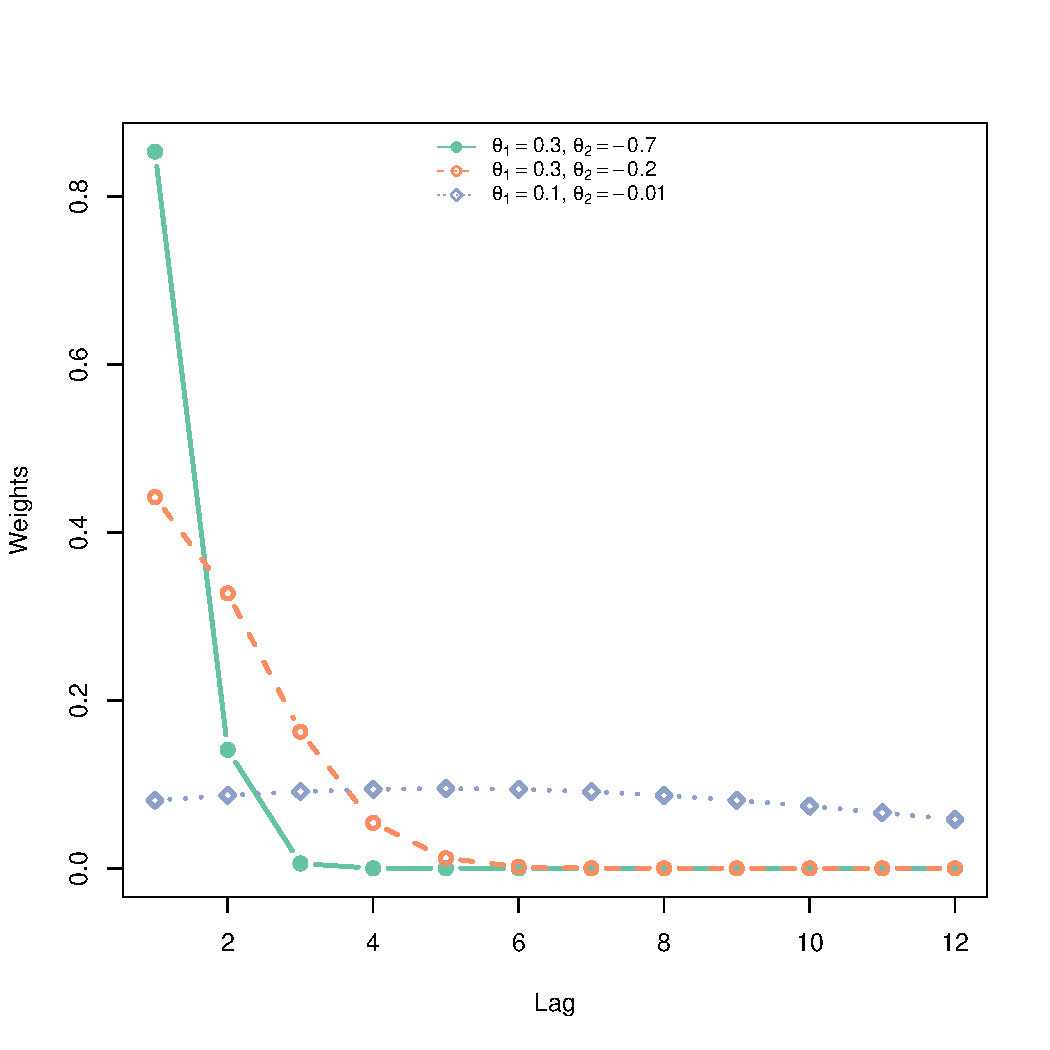
\includegraphics[width=0.5\linewidth]{Figures/weight}
\caption{Weighting schema of exponential Almon Lag function}
\label{fig:weight}
\end{figure}





The resulting model can be estimated by non-linear least squares and used to forecast the target variable from constrained distributed lags of the available data. \cite{Guerin2013}. 


One advantage of such a weighting scheme is that it reduces the dimension of the parameter space and it  extracts information from higher frequency data efficiently. 

One disadvantage of such a weighting scheme comes from imposing arbitrary restrictions on the higher frequency data. For example, exponential Almon lag put positive restriction on the weights for the higher frequency data, which is not necessarily correct \cite{Foroni2013}. The model is susceptible to misspecification. 



\subsection{U-MIDAS weight specifications}

Without a weight scheme, an unrestricted MIDAS regression is similar to an ordinary least squares regressions model which including unconstrained distributed lags of the high frequency predictors.

Consider a two predictors model:

$${y_t= \beta y_{t-1} + \sum_{h=0}^d\theta_{h}x_{tm-h}+\sum_{j=0}^p\phi_{j}z_{tn-j}+u_t}$$

where $m$ and $n$ show $x$ and $z$ have different frequencies.  $h$ and $j$ show $x$ and $j$ have different publication lags. Researchers find that an U-MIDAS model can be easily and fast estimated by OLS. \citeA{Foroni2013} find that if the frequency mismatch is small, U-MIDAS outperforms MIDAS, for example, when mixing monthly and quarterly data. 


\section{State-Space Approach}  

\citeA{Banbura2013} distinguish two types of models for macroeconomic forecasting: partial model and full system methods. 

A bridge equation and a MIDAS model only have a single equation in the model, and can be categorized as a partial model. On the other hand, state-space approach can be categorized as full system model since it involves a system of equations. The system of equations models not only the dynamics of the target variable, but also the dynamics of the predictors. 

\citeA{Bai2013} compare the state-space system model and  MIDAS single equation model. They find MIDAS actually can be represented as a reduced form of a state-space model under some conditions. In most cases, the state-space model gives slight accurate forecast, but state-space model is more computation intensive when the number of predictors is large.  On the other hand, the computation of MIDAS model is straightforward and it can handle a large number of predictors.  


The full system approach includes mixed-frequency VAR, dynamic factor model and factor MIDAS model. This approach uses state space form to handle data with different frequencies. The low frequency target variable is treated as a high frequency one with missing observations. The missing or unobserved latent data can be estimated in a state space model using Kalman filter. 

To deal with the ragged edge data  and prediction problem, this approach uses Kalman filter to model the dynamic of the factors and predict the missing value of factors (VAR is a special case of Kalman filter/ state space model). At the same time, in order to solve the parameter proliferation problem,  some model in this approach use a few factors to capture the information among many predictors. 


\subsection{Mixed frequency VAR}

The vector autoregressive model (VAR) is a great tool to capture co-movement of a set of variables. Instead of a univariate equation, Mixed frequency VAR characterize the co-movements in a system of equations.

\subsubsection{Classical approach} 

A classical approach to estimate the VAR model is maximum-likelihood estimation (MLE) with the expectation maximization algorithm(EM). 

Following the notation of  \citeA{Foroni2014a}, a mixed frequency VAR model with quarterly target variable and monthly predictors can be represented by a state-space model:


\textbf{Transition equation}:

$$s_{t_m} = F s_{t_m-1} + G v_{t_m} \, .$$

$s_{t_m}$ is the state variable at monthly frequency, which can be constructed as follows:

$$s_{t_m} = \begin{bmatrix}z_{t_m} \\ .\\.\\.\\z_{t_m-4}\end{bmatrix}, 
\ \quad z_{t_m} = \begin{bmatrix} y_{t_m}^* - \mu_y^*\\x_{t_m} - \mu_x\end{bmatrix}$$


where $y_{t_m}^*$ is an unobserved latent monthly target variable, $\mu_y= E(y)$, $\mu_y = 3 \mu_y^*$ and $v_{t_m} \sim N(0, I_2)$.  $F$ is a transition matrix. 


\textbf{Measurement equation}:

$$\begin{bmatrix} y_{t_q} - \mu_y \\ x_{t_m} - \mu_x\end{bmatrix}  = H s_{t_m} + \varepsilon_t$$

where $y_{t_q}$ and $x_{t_m}$ are observed data at quarterly and monthly frequencies. $\varepsilon_t$ is a measurement error.

With this state-space representation, the MLE is used to estimation, and Kalman filter is used to forecast.

\subsubsection{Bayesian approach}

Instead of MLE with EM algorithm, the Mixed frequency VAR also can be estimated by Bayesian methods. \citeA{Schorfheide2012} develop a MCMC method for mixed frequency VARs. They use a Minnesota prior for the parameters matrix to deal with the parameters proliferation problem. 

\citeA{BANBURA2014}  and \citeA{Foroni2013}   provide a detailed survey of full system methods, including the Bayesian approach.

\subsection{Mixed-frequency factor model}

In order to avoid parameters proliferation, factor models are  broadly used to summarize information among a large number of predictors.

Factor models decompose time series into a common component, driven by a few factors that represent the key economic driving forces. 

\subsubsection{Factor model}


Consider a regression model with a large number of predictors,

$$y_t = \beta_0 + \beta \mathbf x_t + \epsilon_t, \quad t = 1,\cdots T$$

where  $\mathbf x$ is a $N \times 1$ vector and $N > T$ for a fat regression scenario. $N$ is the number of predictors, and $T$ is the number of observations. This will be impossible to estimate due to the high dimension of the model. With the help of principal component analysis, the dimension can be reduced from $N$ to $q$.  $q$ is the number of the factors. Let:

$$ \mathbf x_{t} = \Lambda \mathbf f_t + \eta_t$$
$$ y_{t} =  \beta_0 +  \beta \mathbf f_{t} + \epsilon_t \,  ,$$

where $\mathbf f$ is $q\times 1$ vector, $\Lambda$ is the factor loading matrix. Traditionally, common factors are estimated by principal components. 

In a static factor model, the relationship be tween $\mathbf x$ and $\mathbf f$ is static , although $\mathbf f$ itself can be a dynamic process. 
 

\subsubsection{Dynamic factor model}

In a dynamic factor model, the relationship between $\mathbf x$ and $\mathbf f$ is dynamic:

$$X_t = \lambda (L) f_t + e_t$$

$$f_t = \Psi (L) f_{t-1} + \eta_t$$

where $X_t$ and $e_t$ are $N \times 1$, $f_t$ and $\eta_t$ are $q \times 1$, $L$ is the lag or lead operator depending on what data we have. The lag polynomial dynamic factor loading matrix  $\lambda (L)$ is $N \times q$, and the lag polynomial transition updating matrix $\Psi (L)$ is  $q \times q$. With this setup, the factors can be used to forecast the target variable using a regression of the target variable on the factors and lagged target variable. 

If $q$ low dimension latent dynamic factors represent the co-movement of a  high dimension vector of $N$ time series $ X_t$,  we can get an efficient forecast for $y_{t+h}$:

$$E(y_{t+h}) = \alpha (L) \mathbf{f_t}  + \delta (L) y_{t}$$

By using aggregated factors as predictors, the dimension of the model is reduced from $N$ to $q$. When we include new variables in $X$, it will not add dimension to  $f$. A dynamic factor model can be represented by a state-space formulation and estimated using the Kalman filter and MLE. The missing values in the ragged edged data  can be handled by an EM algorithm \cite{Stock2006} . 

An alternative solution is a full state-space model approach, which treat low-frequency target variable as a latent monthly data.   

$$X_{t_m} = \Lambda F_{t_m} + \xi_{t_m}$$

$$\Psi (L_m) F_{t_m} = B \eta_{t_m} \, ,$$

where $\eta_{t_m}$ is a $q$-dimensional vector that represents the dynamic factor shocks. The target variable also is treated as a high-frequency variable with missing observations. For example, say, $y_{tm}$ is latent monthly GDP growth. The observed quarterly GDP growth $y_q$ will be treated as the observation in the third month of each quarter, and the other monthly observations are taken as missing.

One disadvantage of the MLE and the Kalman filter for dynamic factor models is when the dimension of $X$  gets very large and there are many parameters needed to be estimated, the MLE becomes unfeasible since it does not have unique solution and the model is not identified.  \citeA{Doz2012}  propose a quasi-ML algorithm to estimate the factors, and then use the Kalman filter  to estimate the unobserved latent monthly factor.  \citeA{Jungbacker2011} show that a transformation of $X$ into low dimension can speed up the calculation of Kalman filter. 


\subsection{Factor-MIDAS}
Given the limitations of a state-space model for dealing with high dimensionality, another popular option is to combine the factor model and MIDAS model. 

Suppose the current information set has high dimensional $N$  predictors $X_{t_m}$. $X_{t_m}$ can be summarized by low dimensional $r$ factors $F_{t_m}$. The most recent available estimated factors $F_{t_m}$ can be used in a MIDAS model. 


The basic Factor-MIDAS approach can be represented as follows: (for simplicity, $r$ is set to equal 1; the target variable is quarterly,the factor is monthly, and the forecast horizon is $h_q$ quarters with $h_q = h_m /3$ )

$$y_{t_q+ h_q} = y_{t_m + h_m} = \beta_0 + \beta_1 b(L_m ; \theta) \hat f_{t_m +w}^{(3)} + \varepsilon_{t_m+ h_m}$$

$$b(L_m ; \theta) = \sum_{k=0}^K c(k; \theta) L_m^k$$

Here, $c(k; \theta)$ is a weighting function, which could be an exponential lag function, or it can be a constant if it is an unlimited MIDAS model. $\hat f_{t_m}^{(3)}$ is skip-sampled from the monthly factor $\hat f_{t_m}$. $(3)$ is the frequency difference. For example, $\hat f_{t_m}^{(3)} =  \hat f_{t_m}, \forall t_m + w = ..., T_m + w -6, T_m + w -3, T_m + w$. With the proper weighting function, the model can be solved by non-linear least squares. 





\section{Shrinkage Methods} 

\citeA{Stock2012} discuss generalized shrinkage methods and show shrinkage methods can handle the high dimension problem just like a factor model. Shrinkage methods include high-dimensional Bayesian vector autoregression \cite{Andersson2008,Banbura2010,Korobilis2013,Carriero2011},  Bayesian model averaging   \cite{Koop2004,Wright2009}, bagging \cite{Inoue2008} , Lasso \cite{DeMol2008,Bai2009} , boosting \cite{Bai2007}, and forecast combination \cite{Timmermann2006}.



\subsection{The LASSO augmented MIDAS} 

To reduce the dimension of the parameter space, factor models  decrease the number of regressors directly. In contrast, penalized regression puts a penalty on the parameters. Penalized regression such as Ridge regression and the LASSO (Least Absolute Shrinkage and Selection Operator) method \cite{Tibshirani1994} have been exploited in the MIDAS approach literature for several years  \cite{DeMol2008,Ferrara2013}.  

\citeA{DeMol2008}  show that for the forecasting of macroeconomic panel data, a Bayesian shrinkage method is a valid alternative to principal components. 

The LASSO augmented MIDAS model can be specified as follows:

$$\hat \beta = \underset{\beta}{\operatorname{argmin}} \displaystyle\sum\limits_{t=1}^T (y_t - \beta_0 - \sum_i^N \beta_i x_{t,i})^2 + \lambda_{lasso} \sum_i^N  |\beta_i|$$

or in matrix form as:

$$\hat \beta =  \underset{\beta}{\operatorname{argmin}}  ||Y-X\beta||_2^2 +  \lambda_{lasso}   ||\beta_i||_1 \, ,$$ 

where $y_t$ is target variable, $x_{t,i}$ is predictors, $\beta$ is the vector of the regression parameters, $N$ is the size of the model, $T$ is number of observations, and $\lambda_{lasso}$ is the tuning parameter which decides how large the penalty is and how sparse the regularization is. Similarly, a Ridge regression comes with a penalty $\lambda_{ridge}||\beta_i||_2$ based on  the norm $\ell_2$,  instead of $\ell_1$. 

The idea behind the LASSO  regression is that the penalty term in optimization process will drive the coefficients $\beta_i$  associated with non-informative predictors $x_i$  to zero and result in a parsimonious model (Ridge regression pushes $\beta_i$ towards to zero, not exactly to zero). The $\lambda$ can be chosen by cross validation. Both LASSO and Ridge regression have Bayesian interpretation. If we assume $\beta_i$ with a prior of a Gaussian distribution with zero mean and standard deviation a function of $\lambda$, then the posterior mode for $\beta_i$ is the Ridge regression solution. If we assume $\beta_i$ with a prior of double-exponential (Laplace) distribution with zero mean and scale parameter a function of $\lambda$, then the the posterior mode for $\beta_i$ is given by the Lasso. \cite{James2013}

\subsection{Model averaging}  
Three popular solutions for ``curse of dimensionality" problem  in the literature are the factor model with principal components; penalized regression with shrinkage; and Bayesian model averaging with variable selection \cite{DeMol2008,Ouysse2013} . These three methods are highly correlated. In some sense, the approach of the factor model and MIDAS model are to aggregate data before forecasting. However, the approach with model averaging is to aggregate the data after forecasting \cite{Hendry2011} . 

Consider a model space consists of $r$ models $M_1, ..., M_r$, and we have the observation data $D$, the prior of $i$th model $P(M_i)$,the prior of the parameter vector in the  $i$th model $P(\theta_i|M_i)$, and likelihood $P(D|\theta_i,M_i)$. The posterior of $i$th model is follows:

$$P(M_i|D) = \frac{P(D|M_i) P(M_i)}{ \sum_{i=1}^{r} P(D|M_i) P(M_i)} \, ,  $$

where 

$$P(D|M_i) = \int P(D|\theta_i,M_i) P(\theta_i|M_i) d\theta_i $$

which is marginal likelihood of the $i$th model. On each $i$th model, we can have a forecast $E(y_{t+1} |D, M_i)$. The weighted average forecast is follow:

$$y_{t+1|t} = E(y_{t+1} |D) = \sum_{i=1}^{r} E(y_{t+1} |D, M_i) P(M_i|D) $$  

\citeA{Timmermann2006}  and \citeA{Stock2009}  provide  a survey of forecast combination methods. When there are $n$ possible regressors, there are $2^n$ possible models in the model space. Searching through the entire model space is very demanding. Furthermore, the parameters might not be time invariant. These issue causes uncertainty and instability of the model. Forecast combinations extract information from all possible forecasting models rather than from a single specific model, which helps to overcome the the problem of model uncertainty \cite{Andreou2013a}. A model ignoring the uncertainty and variability, will not be reliable.Forecast combinations can produce more stable forecasts than individual forecasts, which is useful for dealing with model instability and structural breaks.





\subsection{Bagging and boosting} 

Along with shrinkage method such as Ridge and LASSO, other statistical learning techniques are also used in macroeconomic data analysis. Those methods include ensemble methods like bagging, random forests, and boosting. In the macroeconomics data analysis, Bootstrap aggregation or bagging \cite{Breiman1996} smooths the hard threshold in pre-test estimators by averaging over a bootstrap sample of pre-test estimators.

In terms of the trade-off between bias and variance, bagging can reduce the variance of the estimators significantly without introducing a lot of bias. \citeA{Inoue2008} apply bagging to a forecasting situation and report promising results. \citeA{Bai2009}  discuss three methods: LASSO (least absolute shrinkage and selection operator), LARS (least angle regression), and the elastic net for macroeconomic forecasting.

\citeA{Bai2009}  suggest a way of using boosting to select variables in a factor model setting, and show that some forms of boosting outperform the standard factor-augmented forecasts. \citeA{Buchen2011a} show that boosting is a serious competitor for forecasting US industrial production. \citeA{Carriero2012b}  show that compared to factor models and Bayesian VAR, multivariate boosting performs best when forecasting CPI inflation. \citeA{Wohlrabe2014} also show that boosting outperforms the autoregressive benchmark when forecasting macroeconomic variables for the United States. 


\setlength{\unitlength}{\savedunitlength}